\chapter{Socio-technical systems of \textit{non-core} Drupal projects}
\chaptermark{``Mostly-online" contributions: \textit{non-core} Drupal projects}
\label{sec:custom-to-contrib}

This chapter begins the exploration of different socio-technical systems of contribution activities of the Drupal community. Together with chapter \ref{chapter:core-system}, this chapter will explore the development of Drupal projects, as examples of  ``mostly-online" contribution activities; while chapters \ref{mostly-offline-local:chapter} and \ref{mostly-offline-cons:chapter} will explore the organisation of events, as examples of ``mostly-offline" activities. For each pair of chapters this exploration will start from the most informal socio-technical systems towards the most formal respectively: \textit{custom}, \textit{contributed} and \textit{core} projects, throughout chapters \ref{sec:custom-to-contrib} and \ref{chapter:core-system}; and local events, \textit{DrupalCamps} and \textit{DrupalCons}, throughout chapters \ref{mostly-offline-local:chapter} and \ref{mostly-offline-cons:chapter}.

This chapter also represents the first case used to illustrate the main argument presented during the subsequent four chapters: the growth experienced by the Drupal community led to the formalisation of self-organisational processes in response to a general dynamic of decentralisation of decision-making in order for these processes to scale up. While these organisational dynamics could be interpreted as part of a simple matter of delegation, as in any other large organisation, a significant difference in CBPP communities resides in the peer-based nature of these communities in which ``[...] interaction is not solely or mainly coordinated by contractual relationships, mercantile exchange or hierarchical command. In contrast, individuals are in an autonomous condition" \parencite[11]{p2pvalue-del12:Online}. Hence, the interest for this study lies in how these self-organisational processes emerge, are negotiated, and change over time as the community becomes significantly larger.

Concretely, this chapter explores the emergence and changes experienced over time by socio-technical systems of ``mostly-online" contributions related to the development of Drupal projects that do not form part of the core. These projects represent a rich set of digital commons which has been key for the success and popularity of Drupal, as captured by the popular motto within the community: ``There is a module for that!" \parencite{abbott2016learning}. This relevance is illustrated by the following quote, extracted from a post written by a Drupalista in the blog of a Drupal-specialised company about modules shared on Drupal.org:

\begin{figure}[H]
  \centering
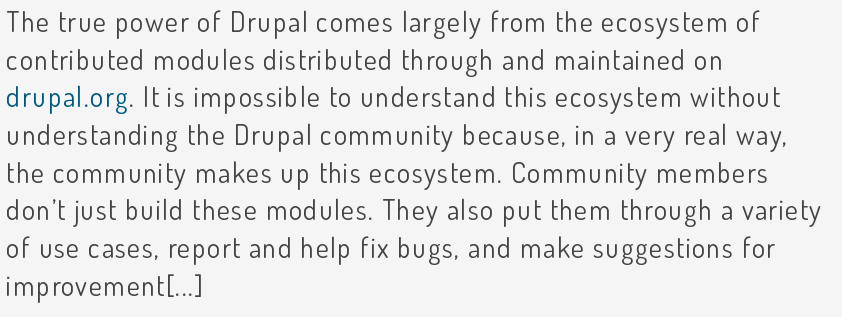
\includegraphics[scale=0.45]{img/quotes_replacement/contrib_ecosystem.png}
\caption[Excerpt from the article ``Introducing Drupal through its community"]{Excerpt from the article ``Introducing Drupal through its community". Retrieved \nth{20} November 2015, from \url{http://www.mediacurrent.com/blog/introducing-drupal-through-its-community}.}
\label{quote_contrib_ecosystem}
\end{figure}

Section \ref{subsec:emergence-contrib} provides an overview of the emergence of systems related to the development of projects that do not form part of Drupal core: \textit{custom} and \textit{contributed} projects. It discusses the significant differences found in their perceived internal value on the basis of whether they are subjected or not to peer-reviewing processes carried out by the community. The process of quality control by which it is decided whether a contributor can obtain permissions to contribute to the socio-technical system of \textit{contributed} projects is more extensively discussed in section \ref{subsec:emergence-pap}. Finally, the chapter concludes presenting an in-depth case study of one of these projects in section \ref{subsec:contrib-day-by-day}, in order to illustrate how the aforementioned dynamics of formalisation and decentralisation operate in the day-to-day.

\section{The emergence of the socio-technical system of \textit{contributed} projects}
\label{subsec:emergence-contrib}

In the early years of Drupal, the transition of a \textit{custom} project into a \textit{contributed} one on Drupal.org was based on an informal process of quality assurance. I\textunderscript{10} and I\textunderscript{9} explained how a single Drupalista used to be responsible for this process, as well as the informality and high degree of centralisation, reflected also in the main collaboration platform at the time:

\begin{quotation}
``[...] at the time [around 2005-2006\footnote{He mentioned later which this occurred between the releases of Drupal 4.6 (15/04/2005) and Drupal 4.7 (01/05/2006).}] the process was, you know, submit a tarball and \textit{John}\footnote{Italics indicate names or nicknames anonymised in the excerpts.} would review it, and if he liked it and it wasn't a duplicate, he would give you commit access to the one [EMPHASISING] CVS repository, that everyone was in. Which meant you had access to commit to every single project in CVS all at once. Oh, yeah... Wild West [LAUGHS]. So that was my start to \textit{contrib} [referring to contribute projects on Drupal.org]."
\begin{flushright}\footnotesize{Drupal core developer and architect, M, 11 years.}\end{flushright}
\end{quotation}

\begin{quotation}
``[...] it was a network of people. And if somebody contributed patches to the project, at some point they were trusted. And they were given CVS access at that time. It was a different version control system, not Git, in that time. So, they just got access to push up to Drupal.org."
\begin{flushright}\footnotesize{Drupal developer and git administrator, M, 8 years.}\end{flushright}
\end{quotation}

Two key aspects from these quotes can be seen as already present during this early stage. Firstly, the action of gaining commit permissions and the perceived value this already had. As will be illustrated in the next sections, this mechanism will be essential to enable the possibility of decentralising decision-making related to the governance and management of these digital commons, while facilitating the scaling up of coordination. In addition, these quotes illustrate the perceived sense of high value which being able to commit --- perform modifications in \textit{official} versions of those digital commons --- had already at the time, in contrast with the lack of internal perceived value associated to \textit{custom} projects not shared within Drupal.org. A high degree of centralisation is also reflected in the technical artefact for collaboration which was employed. CVS is a centralised control version system which was not configured to allow granularity for the definition of permissions for specific projects, and only members belonging or close to that network of people were trusted to perform modifications.

Secondly, these quotes show the existence of rudimentary monitoring mechanisms for projects to be incorporated into Drupal.org as \textit{contributed} projects at the time. As in the case of smaller FLOSS communities, they were based on informal collective choice arrangements: social norms that regulate the expectation of the contributors to create good quality code as a way to generate trust. Those projects that were not subject to these monitoring mechanisms, which in this study are conceptualised as part of the socio-technical system of FLOSS \textit{custom} projects not within Drupal.org, had and have retained perceived low value in the eyes of the members of the community. This shows how whether a project is or is not part of the main collaboration platform has a major impact on the logic of internal value of these digital commons, and how this value is intertwined with the governance and management of these commons. Furthermore, Drupalistas would rarely use \textit{custom} projects not shared within Drupal.org in the sites which they build, which would be considered bad development practice\footnote{Similarly, in the case of requiring to modify files from core when building a website with Drupal, the community encourages Drupalistas to write a patch and share it with the community instead. This practice is illustrated in the well-known motto in the community: ``Never hack core!" \parencite{drupal-never-hack-core:2013:Online}.} \parencite{drupal-contributed:2013:Online}. This aspect contrasts with other FLOSS communities, as explained by I\textunderscript{10}:

\begin{quotation}
``[...] unlike other projects, Drupal.org is the central nexus. If your module isn't on Drupal.org, a lot of people won't touch it, myself included. [...] [for example,] Symfony does not do such a thing [, it] bundles just whatever GitHub repository people feel like using."
\begin{flushright}\footnotesize{Drupal core developer and architect, M, 11 years.}\end{flushright}
\end{quotation}

As the number of contributors and \textit{contributed} projects continued to grow, the result was the emergence of a socio-technical system of \textit{contributed} projects, which is currently composed of thousands of autonomous spaces possessing a higher degree of autonomy and flexibility than those which are part of the core\footnote{The socio-technical system of \textit{core} projects will be extensively discussed in chapter \ref{chapter:core-system}.}. These features are more greatly present in the socio-technical system of \textit{custom} projects shared not within Drupal.org, where no rules regarding quality assurance, coding standards or peer reviewing from the community exist. The perceived lack of value entailed by this leads to Drupalistas greatly favouring the use and contribution to the pool of \textit{contributed} projects, hosted in Drupal.org, a more formalised socio-technical system of contribution. At the same time, the projects which belong to the socio-technical system of \textit{contributed} projects involve a lower degree of coordination compared to \textit{core} projects, as well as to other \textit{contributed} projects within the system itself. The following excerpt by  I\textunderscript{10} illustrates the differences between \textit{core} and \textit{contributed} socio-technical systems:

\begin{quotation}
``[...] Because, they are so different community-wise. I think Drupal core is used by everybody in the community, right? A contributed module is only used by a fraction. Even if that fraction is high, even if 50\% of the sites are using it, the hierarchies are a lot more flexible. They are basically a small group of maintainers, and they make all the decisions, and it's more... chaotic. [...] So, it's just... contributed modules are like small Open Source projects."

\begin{flushright}\footnotesize{Drupal core developer and architect, M, 11 years.}\end{flushright}
\end{quotation}

As part of the emergence and growth of the system of \textit{contributed} projects, extensively discussed in section \ref{sec:growth-community}, the Drupal community had to face questions such as: who should be accountable for accepting and reviewing patches for a \textit{contributed} project? How should it be decided whether a project is included or not? How is it possible to cope with the incremental need to review code?

As a result, the Drupal community formalised these processes in order to scale them up, seeing this dynamic of formalisation reflected in all the relevant entities, such as division of labour and rules from an Activity Theory perspective, that formed part of the analysis carried out in this study. For instance, with regards to the rules that regulate these peer production activities, this was illustrated by the definition of explicit collective-choice arrangements dealing with several aspects such as whether a project should be included or not as \textit{contributed}\footnote{This process is known as Project Application Process, and it will be further detailed in section \ref{subsec:emergence-pap}.}; by establishing explicit processes to request permissions to perform changes in a project in case of abandonment \parencite{maintenance-abadonment:Online}; and by defining a set of expected responsibilities in the form of guidelines for maintainers \parencite{maintenance-guidelines:Online}.

Similarly, numerous examples of the results of formalisation were found in the artefacts employed by the community to facilitate self-organisation. For instance, this is illustrated in the creation of project pages on the main collaboration platform --- see figure \ref{project_page_top} --- that can be interpreted as part of a process to define clearer boundaries, as well as to establish explicit forms of autonomy for decision-making about tasks related to project maintenance. These project pages are under constant negotiation. They experienced changes over time, such as the inclusion of response rates on issues or numbers of open issues (see bottom left corner on figure \ref{project_page_top}), which were found to operate as implicit forms to foster the enforcement of the operational rules negotiated in the community\footnote{Further details on how they operate in this way will be presented in section \ref{subsec:contrib-day-by-day}.}.

\begin{figure}[H]
   \centering
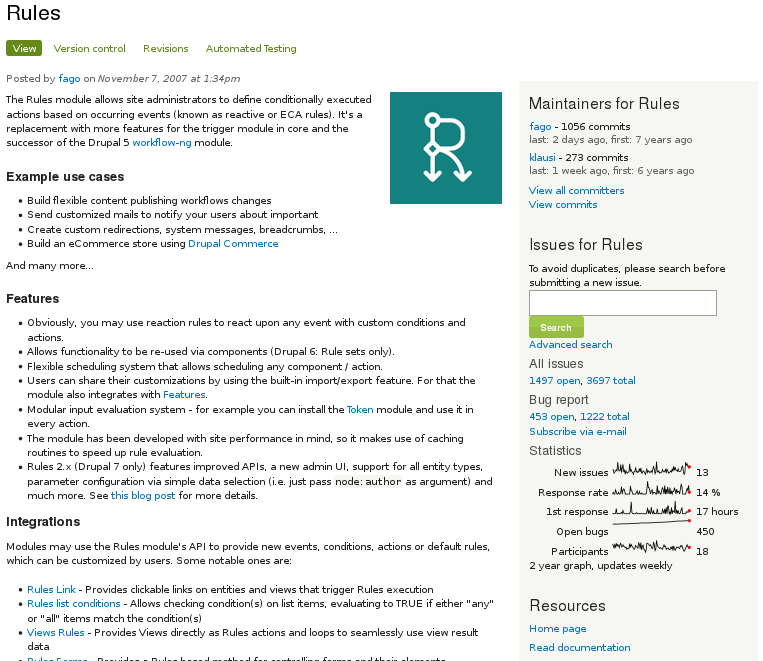
\includegraphics[width=1.0\textwidth]{img/online/project_page_01.png}
 \caption[Project page for a \textit{contributed} Drupal project]%
 {Top section of a \textit{contributed} project page, displaying tools to facilitate the decision-making such as issue lists, clearer jurisdiction in the form of a list of maintainers, as well as statistics related to fostering an implicit enforcement of the operational rules. Retrieved \nth{2} March 2016, from \url{https://www.drupal.org/project/rules}, under a CC BY-SA 2.0 license.}
\label{project_page_top}
\end{figure}

An increasing degree of formalisation was also found in the division of labour and illustrated, for example, by the emergence of explicit and more formal roles. For example, a key role is that of the maintainers --- see upper left corner in figure \ref{project_page_top} --- , who, to obtain this role, must go through different scrutiny processes by the community.

In order to illustrate in wider detail how these dynamics operate in this socio-technical system, the following sections provide further exploration of some of its self-organisational processes. Firstly, the Project Application Process is explored. This is with the aim of further understanding how the dynamics of formalisation and decentralisation occur in the operational rules: how to select those who select, how to make decisions about those who make decisions. Secondly, section \ref{subsec:contrib-day-by-day} presents an in-depth case study of a specific \textit{contributed} project, in order to show how these rules are enforced and how decentralisation in the decision-making for the governance of these digital commons occurs on a daily basis.

\section{The Project Application Process}
\label{subsec:emergence-pap}

As it was briefly introduced in the previous subsection, the Project Application Process (PAP) refers to a quality assurance process carried out by the Drupal community which allows contributors to include a project as part of the socio-technical system of \textit{contributed} projects. Technically, this refers to the obtaining of a ``git vetted role"  by contributors who wish to contribute a project for the first time. This role allows them to administrate this project, create new \textit{official} releases, as well as to create new projects. Once Drupalistas have successfully passed this process, their projects will have a unique name in the main platform of collaboration, with a more visible URL\footnote{An example of the URL of a sandbox project is \url{https://www.drupal.org/sandbox/jcarballo/1990430}. Once a project has become full or official, it will have a url such as \url{https://www.drupal.org/project/fb_likebox}}. I\textunderscript{9}, a git administrator and key member in the organisation of these processes, summarises the current workflow:

\begin{quotation}
``[...] they open an issue on Drupal.org, where they explain the module and [provide a] link to the [sandbox].[...] Which is basically a git repository where you can push any code to. So the thing about those sandboxes is that they don't have a nice URL. They just have a number behind it. So they are not that visible, and they don't have releases. On Drupal.org usually when you go to a project page you can see tag releases which are tarballs of the source code, so that it's easier for people to download. [...] [so when] they want to publish it as a real module under [a] certain namespace [...] they go through the Project Application Process. And then, basically other community members review that code."
\begin{flushright}\footnotesize{Drupal developer and git administrator, M, 8 years.}\end{flushright}
\end{quotation}

Once a Drupalista obtains this role, they can also name other Drupalistas as co-maintainers of their projects. This commonly occurs after Drupalistas interested in that project actively contribute to them, for instance submitting patches, and earn the maintainer's trust. This process illustrates the development of a more formal set of processes for the quality assurance of these digital commons, which provides ways to increase the legitimacy of those Drupalistas governing these digital commons, while facilitating the decentralisation of decision-making with regards to their governance and quality control processes, also making it possible for maintainers to distribute this power. The following excerpt by I\textunderscript{9}, depicts the changes experienced over time with respect to the period previously depicted in section \ref{subsec:emergence-contrib}, in which access to this power depended on the Drupalista's closeness to a single informal network:

\begin{quotation}
``[...] Back in the days in which there was CVS and less contributors it was basically a network thing. So, I know you, you know somebody else, so that person must be trustworthy, let's approve him. Nowadays the process is a bit more formal. So, we have a checklist, basically, which we ran through for the project: are there any licensing issues? Are there any security issues? [...] [is the] API usage in the module really wrong? Or is it otherwise not according to our Code of Conduct of the community? So, basically there's this check that we run through the module. [...] Then, there's a list of people, who are called git administrators on Drupal.org, [however,] anybody can review a module. And they can set it to RTBC, which means Reviewed and Tested By the Community. So anyone can do that. And, after that, a git administrator takes a look, and then approves the account, so they can publish modules."

\begin{flushright}\footnotesize{Drupal developer and git administrator, M, 8 years.}\end{flushright}
\end{quotation}

This is a prominent example of the increasing degree of formalisation in the rules that regulate peer-production in this socio-technical system of contribution. Other examples found were the creation of an explicit consensus-driven check-list \parencite{drupalorg-pap:2016:Online} and the constitution of a set of governance rules which deal with the enforcement of these agreements.

Similarly, the dynamic of formalisation was reflected in the emergence of a clearer and more formalised division of labour within the PAP process itself. For example, it entailed the definition of the explicit figures of applicants, reviewers and git administrators; which also have an explicit formalised set of attributions \parencite{drupalorg-git-admins-01:2016:Online, drupalorg-git-admins-02:2016:Online}, with respect to the rules.

Furthermore, increasing formalisation was reflected in Drupal.org, the main artefact. The clearest example of this being the changes experienced to allow the granular definition of permissions to perform \textit{official} changes in these digital commons and the possibility to easily propagate them. Another example is the use of canonical\footnote{A canonical form is an standarised way of presenting a certain object as a mathematical expression. It determines a unique representation for each of these objects. In this case, the URLs for the projects within Drupal.org.} names for the project that passed this process of quality control, which operates as a means to increase their visibility and internal value. In other words, having a unique and more visible URL after becoming \textit{official} --- or even \textit{real} in the words of I\textunderscript{9} ---,  and the possibility of creating official releases of these projects, are examples of significant factors embedded in the technical artefacts to understand internal logics of value in the community.

Hence it can be observed how, with the need to scale up organisational processes related to the quality assurance of this socio-technical system of \textit{contributed} projects, the Drupal community followed a dynamic of formalisation. This formalisation was reflected in several entities from an Activity Theory perspective such as rules, division of labour and artefacts, which facilitated the decentralisation of decision-making with regards to peer-reviewing, while also acting as a determining factor to define clearer community boundaries.

Driven by a continuous need to scale up these peer-reviewing processes due to the growth experienced, the community discussed and designed initiatives to encourage more people to participate in them. An example of this type of initiatives is the Review Bonus System \parencite{drupalorg-review-bonus-system:2016:Online}, which provides incentives to reduce the waiting period of an applicant for peer-reviewing, after demonstrating proof of having contributed in the peer-reviewing of other projects. In other words, aiming to foster reciprocity. I\textunderscript{9} summarised the initiative:

\begin{quotation}
``[...] to encourage this kind of community spirit that people would help out themselves [...], when we say anyone can review modules... even new applicants, that have freshly joined the project, can review other applicants' code. So that, we can increase the pool of reviewers, basically, and get the sanity check faster for the applicants. [...] the system is called the Review Bonus System, and if you review three other projects, you can add a certain tag to your application, and then it gets to a high priority list, where me, or other git review administrators look regularly. And, we look at those projects first. So, they get approved sooner. Because the problem with the project application in Drupal.org is, of course, that the waiting time is quite long\footnote{A typical review process would commonly take at least two or three months. However, this estimation should be carefully considered as an approximate indicator. It is based on my own experience with the PAP process, comments from Drupalistas in the participant-observation and the interviews, as well as a random inspection of 20 project application issues in the queue at \url{https://www.drupal.org/project/issues/projectapplications?status=7&priorities=All&categories=All&version=All&component=All}. As in previous cases, these figures are included to provide a rough estimation, but they do not provide the accuracy required for a quantitative approach.}."
\begin{flushright}\footnotesize{Drupal developer and git administrator, M, 8 years.}\end{flushright}
\end{quotation}

Initiatives such as this bonus system are sources of tension and intense discussion in the community. For example, in this particular case because the programme entails an additional workload for new contributors, some Drupalistas argue that this impact leads to losing some of these contributors. However, it is also defended by many others, since it represents a way to transfer knowledge, enforce coding standards, and increase reciprocity. For example, discussing his personal experience while going through this process I\textunderscript{7} explained:

\begin{quotation}
``[...] there was a long and hard discussion on how to improve this, because it was a bottleneck. [...] and the idea was that your module is not going to be accepted until you help others. [...] some people started to protest, but I thought it was a brilliant idea. [...] automatically you are helping three more people. Furthermore, you are transferring knowledge among them. [During my application] there were not so many people reviewing modules, so I realised my module would never be accepted unless I helped. So I didn't pay attention to my module for a while, and I started reviewing other people's modules. [...] I read all the documentation and standards, and I learnt tonnes by reading other people's code."
\begin{flushright}\footnotesize{Drupal developer and themer, M, 6 years. Original in Spanish}\end{flushright}
\end{quotation}

The initiative was found to have empowered some Drupalistas to become regular reviewers, and eventually git administrators.  These tensions show the dynamism of these self-organisational aspects, which are under constant negotiation and discussion in the community: to what extent should certain processes be completely open for participation?  Should everyone be allowed to take part in them? While these organisational processes are far from perfect, since the community is continuously struggling to find ways to increase the number of reviewers and git administrators\footnote{At the time of the writing (03/05/2016), the ``Code Review Administrators" (\url{https://groups.drupal.org/node/142454}) Drupal Group listed 32 git administrators, and 500 members. However, these indicators should be carefully interpreted. Regarding git administrators the indicator is more accurate, since changes on the list have been tracked since 2011 (\url{https://groups.drupal.org/node/142454/revisions}). However, regarding the reviewers, the membership to the group indicates simply an interest in it: not all of the reviewers will be members of the group, and some of the group members might not be reviewers. As in previous cases, these figures are included to provide a rough estimation, but they do not provide the necessary accuracy which a more quantitative approach would require.}, they illustrate the continuous seeking of improvement in these self-organisational processes in order to decentralise decision-making. In addition, they have fostered the diversity of Drupalistas carrying out these activities. I\textunderscript{9} explained how this increased decentralisation in decision-making:

\begin{quotation}
``[...] we tried to make the group of git administrators [...] bigger [he sent me the following link \url{https://groups.drupal.org/node/142454}, listing nearly 30 people at the time]. So, it's not only centralised to a couple of people that approve this stuff. So that the group is larger and more people can make this decision. I think that's as decentralised as it can get. If you want to have this kind of approval, you need to have some decision-making at some point, a group of decision makers. [...] [also] we are now more distributed. So, in the former days we were not as diverse as we're now. So, it was mostly people from Europe and the US. While, in git admins we have now also people from other countries. From Africa and from Asia, for example."
\begin{flushright}\footnotesize{Drupal developer and git administrator, M, 8 years.}\end{flushright}
\end{quotation}

Overall, the PAP process illustrates the existence of a dynamic of formalisation in the quality-control mechanisms of this socio-technical system of contribution activities, which enabled the decentralisation of decision-making for the processes of quality control and operational rules to govern and manage these digital commons. The next section provides further detail on how these dynamics of formalisation and decentralisation operate in the maintenance itself, by providing a case study of the day-to-day of a \textit{contributed} project.

\section{Case study: following a \textit{contributed} project}
\label{subsec:contrib-day-by-day}

While the previous sections illustrate the emergence, changes and general organisational dynamics of the socio-technical system of \textit{contributed} projects, there remains a need to offer an in-depth account from a more micro level: how does the day-to-day in the maintenance and governance of these digital commons elapse? How do order and division of labour emerge in such flexible and autonomous spaces? Or, how does the aforementioned dynamic of decentralisation operate at a micro level? To that end, I will draw on my own experience as a project maintainer in the community.

Concretely, the focus will be placed on the story of one of the \textit{contributed} projects I have maintained during the past five years: Facebook Page Plugin or \textit{fb\_likebox}\footnote{See \url{https://www.drupal.org/project/fb_likebox}. The first term refers to the project title, which can be easily updated. Originally, the project title was Facebook Likebox, but was renamed to Facebook Page Plugin for coherence purposes after Facebook changed the name of the widget. The second term refers to the project code, which possesses canonical properties. This project code is employed, for example, for the URL or for the development of code according to the coding standards (e.g. to define custom functions). It is not possible to modify it: renaming requires the creation of a whole new project.}, a small and simple \textit{contributed} project which allows the embedding and configuration of a Page Plugin in a Drupal website using Facebook's API.

\subsection{Origin of \textit{fb\_likebox} and the day-to-day in the maintenance of a \textit{contributed} project}

The story of \textit{fb\_likebox} begins as a conventional one in the Drupal community of a \textit{custom} project becoming a \textit{contributed} one. While I was working for a small company in Madrid as a Drupal developer in 2011, we needed a particular functionality for a project in Drupal 6. I could not find any module with this functionality in Drupal.org, so I created a \textit{custom} one. At that point in time, one year into my life as a Drupalista, I used to attend Drupal events with a certain regularity and I already felt part of the community. I was eager to find as many ways as possible to contribute back to it. This encouraged me to decide to try to contribute my first project to the community. I made the project more generic and I extended some of its functionalities during my spare time. In order to publish it in Drupal.org as a \textit{contributed} project, I had to pass the PAP process, previously presented in section \ref{subsec:emergence-pap}, which I started in August 2011. After several months of reviewing requested changes in the sandbox\footnote{See \url{https://www.drupal.org/node/1257326}.}, it became an official module in Drupal.org\footnote{See \url{https://www.drupal.org/project/fb_likebox}.} in November 2011 --- see figure \ref{fb_likebox}.

\begin{figure}[H]
    \centering
    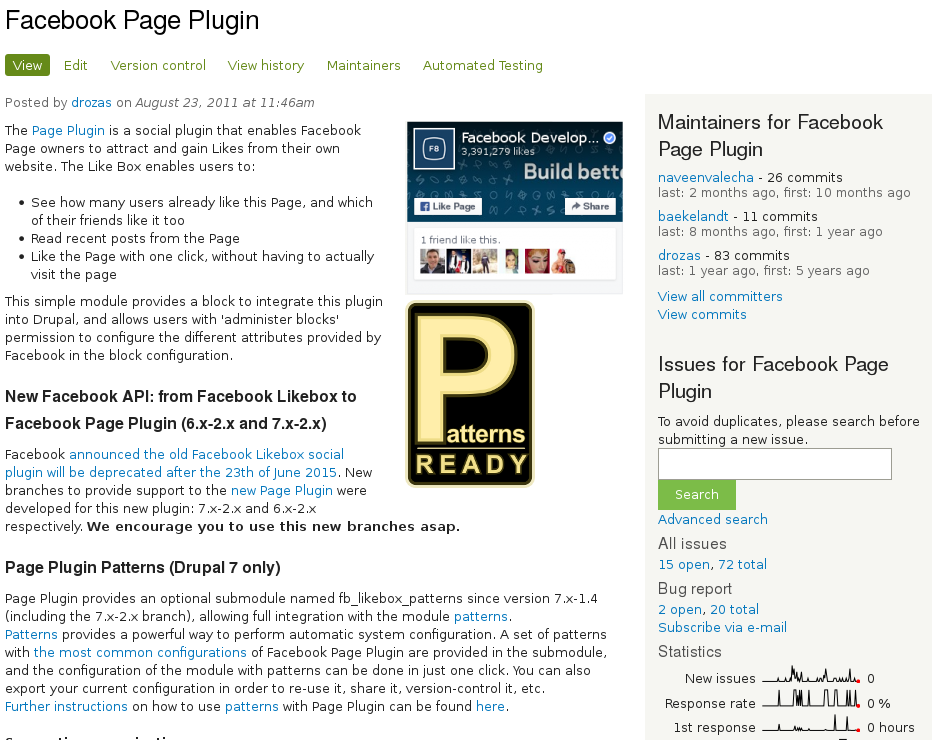
\includegraphics[scale=0.42]{img/online/fb_likebox.png}
     \caption[Facebook Page Plugin project page at Drupal.org]%
     {Official Facebook Page Plugin project page at Drupal.org. Retrieved \nth{6} October 2016, from \url{https://www.drupal.org/project/fb_likebox}, under a CC BY-SA 2.0 license.}
     \label{fb_likebox}
\end{figure}

Although \textit{fb\_likebox} is a small and simple module, it became relatively popular in terms of number of installations\footnote{See \url{https://www.drupal.org/project/usage/fb_likebox}. At the time of writing (October 2016), it had 12,915 installations, ranking it as \nth{428} (\url{https://www.drupal.org/project/usage?page=4}) out of the 18,364 \textit{contributed} projects in Drupal according to Drupal.org's statistics for site installations.}. It surpassed the 1,000 installations mark in November 2012, and the 10,000 installations mark in May 2015 after releasing a Drupal 7 version.

As a maintainer of a \textit{contributed} project in Drupal.org, I could personally experience the satisfaction of feeling that your work can be useful for other people, in line with some of the common intrinsic motivations by FLOSS developers discussed in section \ref{subsubsec:state-art:floss:academic-research}. Additionally, I experienced the effect which certain characteristics of the main artefacts of collaboration have to work as a motivator, increasing my commitment with the maintenance of the project\footnote{Projects in Drupal.org are generated through a Drupal module called Project (\url{https://www.drupal.org/project/project}), which provides a content type and functionalities with tools for management. Discussions about data collection, such as what indicators to show and within which ranges, are reflected on the Project module issues list (1,779 issues at the time of writing, October 2016) in which every Drupalista can participate --- \url{https://www.drupal.org/project/issues/project?status=All&categories=All}.}. For example, I used to check the statistics of the number of site installations of my \textit{contributed} projects once a week, when they were refreshed in Drupal.org, and I experienced a great satisfaction in seeing these figures constantly increase. In addition, some of the changes in the project pages of Drupal.org, such as the inclusion of public statistics (e.g. response rate or number of unresolved bugs, as shown in figure \ref{fb_likebox}), created a form of socio-technical pressure in me to try to always keep the module updated and respond to issues as soon as I could. For example, although there are not any specific rules regarding this matter, I felt I had the responsibility to give prompt replies to Drupalistas opening issues in less than 24 hours, as this would be perceived as a sign of being a ``responsible maintainer", and my ``good behaviour" as a Drupalista would also be reflected in these public statistics.

My reactions towards these indicators was due to both my intrinsic motivation for ``doing good for the commons", but also my extrinsic motivation to have a good reputation as a contributor, which is important for my career as a professional Drupal developer. The increasing pressure instilled by more formal mechanisms added over time, however, is also seen by some Drupalistas as placing even more responsibilities on the shoulders of Drupalistas who are already subjected to a large set of expectations. For example, Drupalistas maintaining several projects complained about having an almost perpetual responsibility in the eyes of the community for sharing the code in the first place. The following excerpt by I\textunderscript{5}, who maintains several projects, illustrates this view:

\begin{quotation}
``[...] maintaining a module becomes sometimes a bit like a `life sentence'. Because when you propose your code, and publish it... sometimes it seems you're signing some sort of `lifetime warranty' to maintain it. And that's because we don't have a clear process."

\begin{flushright}\footnotesize{Drupal developer and ex-member of the Drupal Association Board of Directors, M, 9 years. Original reply in Spanish.}\end{flushright}
\end{quotation}

This quote shows how these organisational processes, despite having become more formalised over time as shown in the previous section, still possess aspects of informality, which, in the case of this Drupalista, was experienced as frustration at a lack of clarity. Changes in the artefacts, as those previously discussed, can be understood as informal forms of enforcement in the community, in this case intended to increase the commitment of the maintainer through the idea of reputation: ``you are expected to take care of the module and keep a clear and active issue list". These forms of informal enforcement are also reinforced by the ``do-ocratic" culture of the community, in similar ways as in other spaces regulated by hacker culture \parencite{levy1984hackers, coleman2013coding} which promotes the creation of high quality source code. Despite this, these spaces are largely autonomous, and the day-to-day enforcement of the implicit rules depends on the willingness of the maintainers.

This is a relevant aspect for the understanding of self-organisation in CBPP communities and for their sustainability. Since these communities are based on peer relationships, meaning interactions are not mainly based on contractual relationships \parencite{morell2016mayo}, the establishment of a ``do-ocratic" culture to foster contributions to the commons therefore plays a significant role. This culture is constructed through the notion of contribution, a notion that is constantly fostered and is intertwined with that of reputation in the community. For example, at an individual level, in the case of \textit{contributed} projects this is seen through the idea of encouraging the contribution of well-designed, useful and popular projects, whose quality and value are under the continuous scrutiny of the community. This also operates with macro organisational aspects, for example, with regards to the notion of internal value. If there are several ways to satisfy a certain functionality by several \textit{contributed} projects, or combinations of them, it is common practice to inspect the open statistics of the project at Drupal.org to choose one with more active maintenance, as a sign of reliability. Furthermore, in the view of some Drupalistas, this socio-technical system of contribution is based on the ``survival of the fittest", in which projects that are not properly maintained or whose functionalities are more efficiently fulfilled by others, will eventually lack installations, and will be organically deprecated. The following quote, extracted from a blog post written by a Drupalista in the blog of her company, illustrates this common view:

\begin{figure}[H]
 \centering
 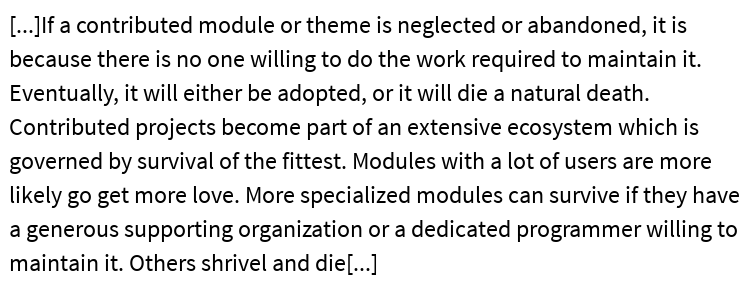
\includegraphics[scale=0.5]{img/quotes_replacement/quote_nerdery.png}
	\caption[Excerpt from the article ``Do-ocracy and the Drupal \textit{Contrib} Ecosystem"]{Excerpt from the article ``Do-ocracy and the Drupal \textit{Contrib} Ecosystem". Retrieved \nth{7} October 2016, from \url{https://nerdery.com/blog/do-ocracy-and-the-drupal-contrib-ecosystem}.}
   \label{quote_nerdery}
\end{figure}

Nevertheless, the ``survival of the fittest" nature of this socio-technical system of contribution is better understood as one based on co-opetition \parencite{brandenburger2011co} than on competition, as found in other FLOSS communities \parencite{west2006patterns, teixeira2014understanding}. The social norms of the community encourage collaboration in existing projects and joining forces, rather than competing \parencite{maintenance-guidelines:Online}, with the additional aim of reducing duplication. Even in cases in which several \textit{contributed} projects offer similar functionalities, whose co-existence in the main collaboration platform must be successfully justified and approved during the PAP process, and they do compete, this is understood within the community as a healthy form of competition, a source of innovation, and an opportunity to find ways for future collaboration. Picture \ref{compiting} depicts two Drupalistas maintaining competing projects and expressing this competitive feeling in a humorous way during their encounter at a Drupal event, which is in congruence with the previously described use of humour in hacker culture \textcite[116]{coleman2013coding}.

\begin{figure}[H]
   \centering
    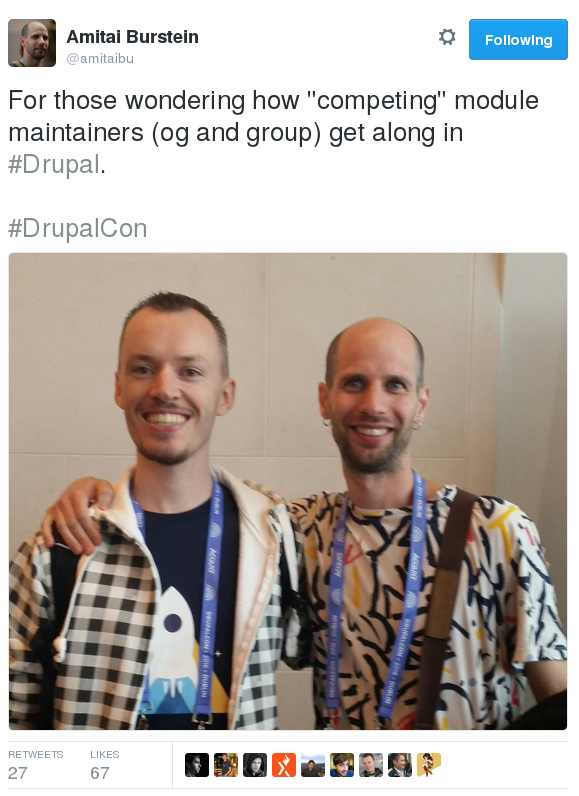
\includegraphics[scale=0.4]{img/online/coopetition.png}
    \caption[Tweet from a Drupalista with his ``competitor"]%
    {Tweet from a Drupalista with his ``competitor". In the subsequent tweets some Drupalistas encouraged them to join forces. Retrieved \nth{11} October 2016, from \url{https://twitter.com/amitaibu/status/780710566193225728}.}
    \label{compiting}
\end{figure}

On the other hand, the previous quote by I\textunderscript{5}, also shows how the remaining highly informal character of this socio-technical system of contribution, manifested in this case through a lack of clear responsibilities, in conjunction with these elements of `do-ocratic' culture which surround the processes, also constitutes a source of tension on certain occasions with respect to the self-allocation of tasks. For example, regarding the expectations on maintainers to develop new functionalities or solve bugs. Drupalistas often identified the source of these tensions as other Drupalistas', especially newcomers', lack of understanding of how FLOSS communities work: those who are not familiar with the culture of the community tend to behave more as customers than as part of the community, thus displaying a lack of internalised responsibility to contribute to maintenance, as expected in the community. The following excerpt by I\textunderscript{7} shows the internalisation of these values, and how the ``do-ocratic" culture of the community, which promotes taking an active role, is extended even as part of the professional practices of Drupalistas:

\begin{quotation}
``[...] so you publish your module, and then people start using it. And some of them report bugs, or ask for new functionalities: `it would be great if your module does this or that'. And then... what happens? Well, there's a guide for module maintenance... and you're expected to follow certain guidelines, you're expected to reply if someone asks, if someone opens an issue, a bug or whatever. But, sometimes you find people who don't understand free software. It's almost as if they were your customer. And things don't work like that. [...] as an unwritten rule in the community, the idea is that if you're using a certain module, and you detect a bug, you should try to solve it. [...] For example, as a coordinator in my company, in my team this is something I require from the developers I work with: `if you see a problem, write a patch and contribute it via an issue. Afterwards, you can worry about integrating it in our project, or wait until it's committed by the maintainer'. But that's the first thing: talking to the maintainer."
\begin{flushright}\footnotesize{Drupal developer and themer, M, 6 years. Original in Spanish}\end{flushright}
\end{quotation}

My first years in the maintenance of \textit{fb\_likebox} elapsed within this environment of sporadic contributions described by I\textunderscript{7}. Some Drupalistas reported bugs or asked for new features via the issues list\footnote{See \url{https://www.drupal.org/project/issues/fb_likebox?status=All&categories=All}.}. I used to take care of these issues during my spare time, especially at code sprints at Drupal events, as those presented in section \ref{sec:growth-community}. On some occasions, some Drupalistas provided patches to the code to solve bugs or to include new functionalities. I inspected and tested the patches or comments, and I provided attribution to the contributor while carrying out the commit if I considered the contribution was valuable enough. In this way, they would appear as committers on the project page\footnote{See \url{https://www.drupal.org/node/1257306/committers}.}, and these contributions were also reflected in their user profiles. During my first years as a maintainer, this process of attribution was encouraged as part of the guidelines for maintainers, but it required a tedious manual search of the unique identifiers\footnote{In order to provide attribution, the message of the commit had to include the usernames of all the contributors, as well as the authorship of one of them which required locating the identifier (e.g. --author=``jonhdoe \textless johndoe@8389.no-reply.drupal.org\textgreater". Previous versions of the documentation \parencite{credit-cvs:Online} provide an overview of how the process of attribution used to work.} of the Drupalistas in their profiles before carrying out the commit. However, subsequent versions of Drupal.org included a functionality to encourage and facilitate attribution, by automatically retrieving data from Drupalistas who participate in the issue --- see figure \ref{fb_likebox_credit} --- and creating an automatic message for the commit to set this attribution. This example reflects how the previously discussed ``do-ocratic" values are progressively more embedded and formalised in the technological artefacts employed by the community.

\begin{figure}[H]
     \centering
   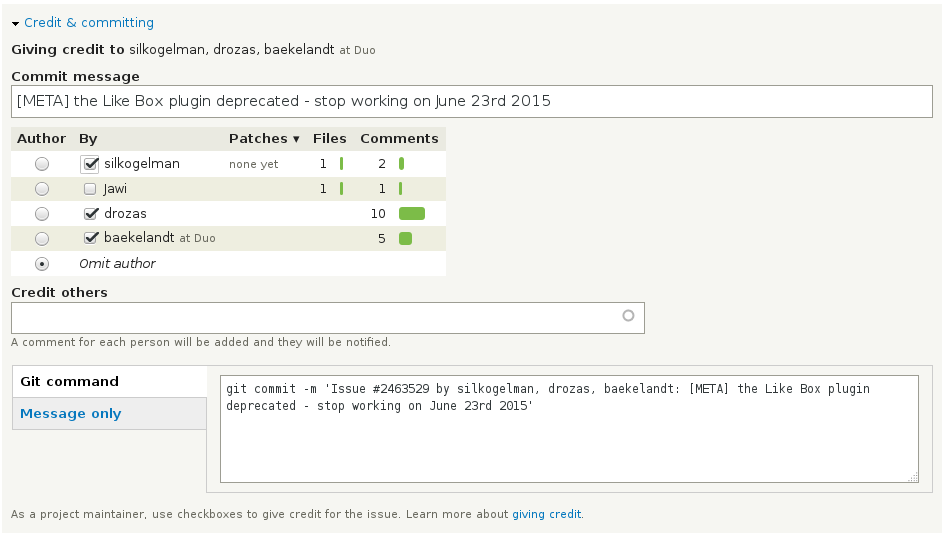
\includegraphics[scale=0.42]{img/online/fb_likebox_providing_credit.png}
    \caption[Providing credit in Facebook Page Plugin]%
        {Example of the changes related to providing credit in the artefacts for collaboration for the development of projects. Retrieved \nth{7} October 2016, from \url{https://www.drupal.org/node/2463529https://www.drupal.org/node/2463529}, under a CC BY-SA 2.0 license.}
    \label{fb_likebox_credit}
\end{figure}

Overall, the previous excerpts illustrate the high degree of organicity and autonomy of the organisational processes in this socio-technical system of contribution, and how in certain cases, some of these projects ``co-ompete" with each other. Although the system was subjected to a general dynamic of formalisation, the day-to-day for its regulation and enforcement still depends more on the community's implicit social norms. This day-to-day activity is intertwined with technical artefacts that encourage active maintenance via open statistics in the platform to foster the mix of intrinsic and extrinsic motivations of maintainers, who also act as a large set of distributed gatekeepers who carry out quality assurance processes and have the power to acknowledge the value of contributions provided by other Drupalistas by reflecting them in these technical artefacts.

\subsection{A story of decentralisation in a \textit{contributed} project}

A subsequent set of events which occurred with \textit{fb\_likebox} provides a valuable way to understand how decentralisation organically happens in these environments. As a maintainer, I used to receive sporadic contributions for this module up to early 2015: some Drupalistas provided feedback and patches on certain occasions. I reviewed and tested their contributions, and I incorporated them and provided credit to the contributors if I considered their contributions valuable enough. However, during this stage contributors tend to come and go.

Nevertheless, in May 2015 one of them became a regular contributor\footnote{See \url{https://www.drupal.org/user/3157937/track/code}.}. His collaboration started as part of an issue which I opened some months before, when Facebook announced\footnote{See \url{https://developers.facebook.com/docs/plugins/like-box-for-pages}.} they would change their API and deprecate the old one in late June 2015, requiring major changes in the \textit{contributed} project. This Drupalista explained to me that he had started working on the changes of the code, and we moved part of our discussions to e-mails on some occasions, while we also kept using the issues list to make the activities transparent allowing other Drupalistas to participate.

The field notes from those weeks reflect how I also experienced a sense of connection with this Drupalista while collaborating, which relates to the affective labour discussed in section \ref{subsec:insights:affective-labour}. We built a shared experience of becoming a small team within this autonomous space. For instance, we organised ourselves to review patches from other contributors, or discussed what the priorities of the project should be, while sharing jokes online, or discussing drinking a beer together at a future Drupal event if we could both attend. After some weeks, I offered him the possibility of becoming a co-maintainer of the project. The excerpt below, extracted from our e-mail exchange, illustrates how, through these interactions, this Drupalista became more empowered --- it was his first time contributing code --- and how he felt the project was also his:

\begin{figure}[H]
    \centering
 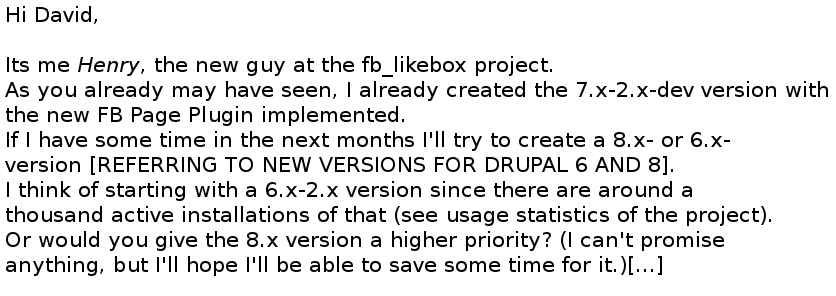
\includegraphics[scale=0.5]{img/quotes_replacement/quote_henry_email.png}
  \caption[Excerpt extracted from an e-mail sent by \textit{Henry}]{Excerpt extracted from an e-mail received on \nth{21} May 2015.}
   \label{quote_henry_email}
\end{figure}

As discussed in the previous section, the changes in the main collaboration platform allow these permissions to be propagated: once you become a co-maintainer of a certain module, you can also grant the possibility of becoming co-maintainer to other Drupalistas. During the next months I was able to observe how, as part of this initial step towards the decentralisation of decision-making and emergent team spirit, the group became larger, more active and the responsibilities more distributed. As a single maintainer, I used to take all the decisions by myself. However, at this point the decisions about the direction of this small module were made by a small ``core" of Drupalistas interested in Facebook Page Plugin. Furthermore, the possibility of propagating permissions was employed by \textit{Henry} to make another Drupalista, who expressed his intention of porting the module to Drupal 8\footnote{See \url{https://www.drupal.org/node/2656166}.}, a co-maintainer. Hence, showing how the changes carried out in the main collaboration platform facilitated the possibility for the power to commit to be more distributed, and to be propagated by others, as \textit{Henry} did.

During this period, ranging from May 2015, in which I named \textit{Henry} co-maintainer, to the time of writing (October 2016), the module moved from 1 to 3 maintainers\footnote{See \url{https://www.drupal.org/node/1257306/maintainers}.}, the number of committers increased from 4 to 11\footnote{See \url{https://www.drupal.org/node/1257306/committers}.}, and tens\footnote{See \url{https://www.drupal.org/project/issues/fb_likebox?text=&status=All&priorities=All&categories=All&version=All&component=All}.} of Drupalistas participated and self-organised through the issues list to test patches, improve the documentation, or even discuss whether we should change the name of the module and the project code after Facebook's changes in the API\footnote{See \url{https://www.drupal.org/node/2700877}.}. For example, picture \ref{fb_likebox_meta} depicts the creation of a meta issue\footnote{Meta issues are an extended practice in the Drupal community to organise complex tasks, such as a whole new version, into smaller ones. They are also a common point at which the direction of that specific part of the project is discussed by the participants.} by the third co-maintainer regarding the development of a new release for Drupal 8, the development of which was led by him.

\begin{figure}[H]
   \centering
   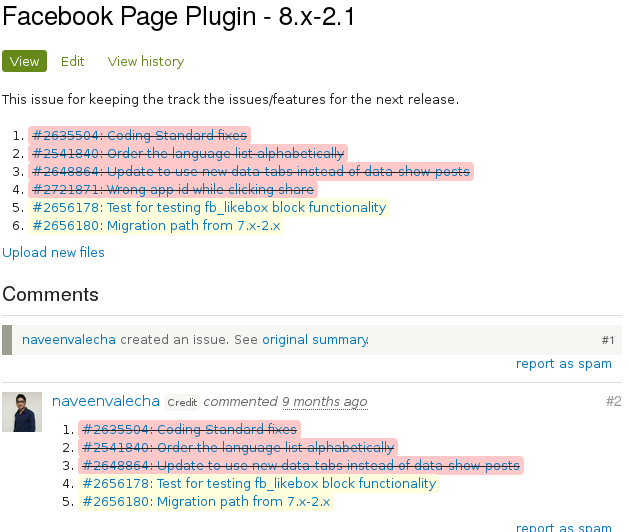
\includegraphics[scale=0.55]{img/online/fb_likebox_8_meta.png}
    \caption[Meta issue in Facebook Page Plugin]%
   {Partial screenshot of a meta issue for Facebook Page Plugin to organise the tasks to port the module to Drupal 8. Retrieved \nth{7} October 2016, from \url{https://www.drupal.org/node/2656166}, under a CC BY-SA 2.0 license.}
\label{fb_likebox_meta}
\end{figure}

Even in the case of a small module such as \textit{fb\_likebox}, these experiences illustrate how decentralisation of decision-making occurs in this socio-technical system of contribution. Over the course of this period, I could observe how Drupalistas became empowered to take part in decision-making regarding the direction of the project, the quality assurance processes, or even the possibility to change the whole identity of the project itself, among others. The case of the presented module is not unique, the collected data show how this is a common case. For example, the following excerpt by I\textunderscript{9}, a Drupalista with much experience in this socio-technical system of contribution and one of the key Drupalistas in the PAP process, depicts how this case is common in the community:

\begin{quotation}
``[...] I think that the community involvement is bigger [in Drupal] than in other Open Source projects. In other Open Source projects, especially the small ones, there's most of the time one maintainer. And one maintainer manages everything, reviews patches, gives feedback, and there's a wider community around that which submits those patches or pull requests. But the ultimate decision only one maintainer makes. In Drupal most of the time there are several maintainers, there are more active community members that review more, so... there are more roles, [...]. So there are not only the maintainers, there are roles in between [...] and, at some point they might become maintainers themselves. [...]"
\begin{flushright}\footnotesize{Drupal developer and git administrator, M, 8 years.}\end{flushright}
\end{quotation}

Overall, this socio-technical system of contribution can be thought of as a large set of autonomous spaces, which can be conceptualised as small hubs of coordination, with an organic division of labour, and in which thousands of centres of decision-making, as in the case of \textit{fb\_likebox}, emerge. The day-to-day in this socio-technical system of contribution is regulated and characterised by having a high degree of autonomy and flexibility; and in which, although the legitimacy to carry out decision-making and the responsibilities to maintain and govern these commons have been more formalised over time, there remains a considerable degree of informality in the actions and processes by which these commons are regulated. Far from formal duties, the enforcement of rules and the sustainability of these digital commons rely on Drupalistas' sense of self-responsibility, which is encouraged by the ``do-ocratic" values of the community and reflected and fostered by the main artefacts for collaboration.

\section{Conclusion}

Throughout this chapter the study of self-organisational processes of a large and global CBPP community began, focussing on the study of the development of \textit{non-core} projects. Around these contribution activities two socio-technical systems emerged: one composed of \textit{custom} projects not within the main collaboration platform, characterised by their perceived low internal value in the eyes of Drupalistas due to the lack of quality control. Secondly, one composed of \textit{contributed} projects that form part of the official platform, which experienced an increment in the degree of formalisation in their organisational processes, which was argued to have facilitated the decentralisation of decision-making with regards to their governance. Subsequently, the general processes of quality control as well as those related to the regular maintenance of these digital commons were more extensively explored, shedding light on how these self-organisational processes and the internal logics of value of the community are intertwined in the day-to-day.

Overall, the socio-technical system of \textit{contributed} projects represents a more valued system than that of \textit{custom} projects shared not within Drupal.org. This revealed how whether a project is subject to communitarian quality control mechanisms has a major impact on the perceived value of these contributions from Drupalistas, also affecting the use of \textit{custom} projects by Drupalistas in the day-to-day when building sites with Drupal. Overall, the socio-technical system of \textit{contributed} projects represents an autonomous and flexible organisational environment, which acts as a source of innovation and experimentation in the community, and facilitates the participation and empowerment of Drupalistas to contribute for the first time, as in the case of \textit{Henry}, or myself. 

However, the socio-technical system of \textit{contributed} projects is also a more chaotic and uncoordinated socio-technical system when compared to other socio-technical systems in the community, such as that of the development of \textit{core} projects; suffering with problems of duplication, wasted resources, a lack of consistency, and the absence of reliability in certain cases. It is precisely to this socio-technical system of \textit{core} projects that the focus will be shifted in the next chapter, with the aim of continuing the exploration of the general dynamics of formalisation and decentralisation in decision-making. This also allows the comparison between the different degrees of formalisation and decentralisation, and the way in which the identified dynamics affected the self-organisational processes, despite both systems being focussed on the same type of object --- source code in the form of Drupal projects --- as well as both belonging to the ``mostly-online" side of the spectrum with regards to the main medium.